\chapter{Background}\label{chap:background}
\thispagestyle{plain}
\newglossaryentry{LLM}{
    name={LLM},
    description={Large Language Model},
    symbol={LLM},
    sort={LLM}
}

\section{Github}
GitHub is an online platform built on Git, a distributed version control system, designed to streamline IT project management and team collaboration. It is a go-to solution for source control and teamwork in software development, accommodating projects of any scale. By integrating Git's capabilities, such as version tracking and distributed repositories, with an easy-to-use interface, GitHub simplifies the adoption process for developers of all skill levels. The platform also includes advanced features that enhance teamwork and organization, such as access controls to regulate viewing and editing permissions, bug tracking for error management, and tools for suggesting and discussing new features. Additional functionalities, like task management, wikis for centralized documentation, and sophisticated pull request workflows, enable structured code reviews and seamless integration of changes. These attributes make GitHub more than just a tool; it is a collaborative environment that promotes transparency, innovation, and efficiency, earning widespread adoption by developers and organizations globally.
\subsection{Commit}
"In version control using Git, the commit mes- sage is a document that summarizes source code changes in natural language." \citet{jung-2021-commitbert}.
 A well-structured message helps developers to track changes in chronological order and quickly understand their content. For this reason, it is always a good idea to write clear and meaningful commits, so as to facilitate the management and review of the code over time.
\subsection{Pull request}
A pull request serves as a critical mechanism for contributing to software projects, particularly in collaborative or open-source environments. It enables contributors to submit changes to a project's source code through an intuitive interface, allowing team members to review, discuss, and merge those changes in a controlled and systematic way, thereby reducing the likelihood of errors. "But, the pull request is more than just a notification—it’s a dedicated forum for discussing the proposed feature. If there are any problems with the changes, teammates can post feedback in the pull request and even tweak the feature by pushing follow-up commits. All of this activity is tracked directly inside of the pull request."\citet{atlassian_pull_request}. Every activity, including reviews, comments, and code updates, is documented and centralized, ensuring transparency and accountability. Additionally, pull requests provide essential information, such as the commits involved, linked issues, and detailed code differences (diffs), supporting a structured and thorough review process.
\begin{figure}[H]
  \centering
  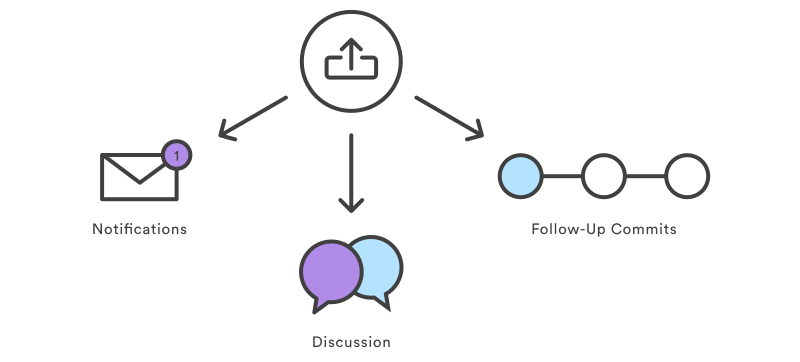
\includegraphics[width=\textwidth]{figures/02.png}
  \caption{Representation of a pull request. Source: Atlassian (2025)\citet{atlassian_pull_request}.}
  \label{fig:pull_request_image}
\end{figure}

\section{Large language model}
A large language model (LLM) is an advanced technology developed to understand and generate text in complex and diverse contexts. Its operation is based on the processing of huge amounts of textual data, which allows the model to learn a large number of parameters during the training phase. These models exploit advanced machine learning techniques, such as transformative neural networks, to produce coherent and relevant responses. However, their design and use require considerable computational resources, both in terms of training time and execution time, making them expensive and complex to manage. Due to their versatility, large language models find application in multiple areas, such as content generation, machine translation, and programming support, demonstrating their ability to tackle complex problems related to natural language.
\subsection{Prompt Engineering}
Prompt engineering is an emerging discipline that arose in parallel with the development of large language models (LLMs). It is the art of designing and structuring prompts effectively to optimize the responses generated by the model, maximizing their utility in solving specific tasks and in research activities.
When developing and testing prompts for an LLM, you can interact with the model directly or through an API. In the latter case, you can adjust some parameters that influence the behavior of the model, allowing you to adapt the answers to specific needs. Optimizing these settings is essential to improve the quality, reliability, and relevance of the generated answers. However, finding the ideal configuration requires experimentation and adaptation based on the context of use.
\newline
\subsubsection{Key parameters in LLM configuration}
\textit{Temperature}:\newline
This parameter controls the level of randomness in text generation. A low value makes the model more deterministic, favoring consistent and predictable answers based on the highest probabilities. Conversely, a high value introduces more variability, encouraging more creative and diverse answers. For example, in fact-based question answering applications, it is preferable to keep the temperature low to ensure precise and concise answers. For creative tasks such as poetry writing or idea generation, increasing the temperature can lead to more original and less rigid results.
\newline
\textit{Maximum length}:\newline
Defines the maximum number of tokens that the model can generate in a response. Limiting this parameter helps control the length of responses, avoiding excessively verbose or out-of-context output. Furthermore, effective length management allows you to optimize computational resources and reduce costs related to the use of the model.
\subsubsection{Types of prompts}
\textit{Zero-shot}:\newline
A zero-shot prompt is a type of prompt where the model is not given any training examples before generating a response. The model is instructed to respond directly to the prompt, relying on its general knowledge and understanding of the language.\newline
\textit{One-shot}:\newline
A one-shot prompt provides a single example of how the model should respond, along with the prompt. In other words, the model receives an input-output example, which helps it better understand the specific task before generating the response.\newline
\textit{Few-shot}:\newline
A few-shot prompt provides the model with a few examples of input-output. Unlike a one-shot, a few-shot contains more than one example, usually 2 to 5. The model then receives a series of examples that allow it to learn the task and respond more accurately.
\section{Use Case: Automatically Generate Pull Request Messages}
In collaborative software development, managing pull requests (PRs) is essential. Each pull request includes essential metadata such as the title, message body, associated commits, code changes (diffs), and associated issues. Writing descriptive and meaningful PR messages is a subjective task and can vary in quality and detail among contributors.
\subsection{Problem}
\begin{itemize}
\item The quality of pull request messages can negatively impact code review, slowing down decision-making and increasing the risk of errors.
\item Writing messages manually is time-consuming and may not meet documentation standards, especially in distributed or open source teams.
\subsection{Use Case Goal}
Use a \textit{large language model (LLM)} by providing it with a specific dataset, integrating \textit{metadata} and \textit{code changes}, to automatically generate accurate, clear, and informative pull request messages such as title or body message.
\subsection{Usage Flow}
\subsubsection{Body Message Generation}
\begin{enumerate}
\item A contributor creates a pull request on a GitHub repository.
\item The system collects data about the pull request, including:
\begin{itemize}
\item The proposed title.
\item The changes to the code (\textit{diff}).
\item Any associated issues with comments from contributors.
\end{itemize}
\item The LLM processes this data as input and generates:
\begin{itemize}
\item A detailed message body highlighting the changes, reasons, and impacts.
\end{itemize}
\item The result is returned to the user, who can accept, edit, or improve it.
\end{enumerate}
\subsubsection{Title Generation}
\begin{enumerate}
\item A contributor creates a pull request on a GitHub repository.
\item The system collects data about the pull request, including:
\begin{itemize}
\item The body message.
\item The commit message.
\item The changes to the code (\textit{diff}).
\end{itemize}
\item The LLM processes this data as input and generates:
\begin{itemize}
\item A descriptive title for the pull request.
\end{itemize}
\item The result is returned to the user, who can accept, edit, or improve it.
\end{enumerate}
\end{itemize}
